\question Q3\droppoints

\begin{solution}
    \text{(a) - (f), (h) - (k)} Implemented.

    \text{(g)}

    \centerline {
        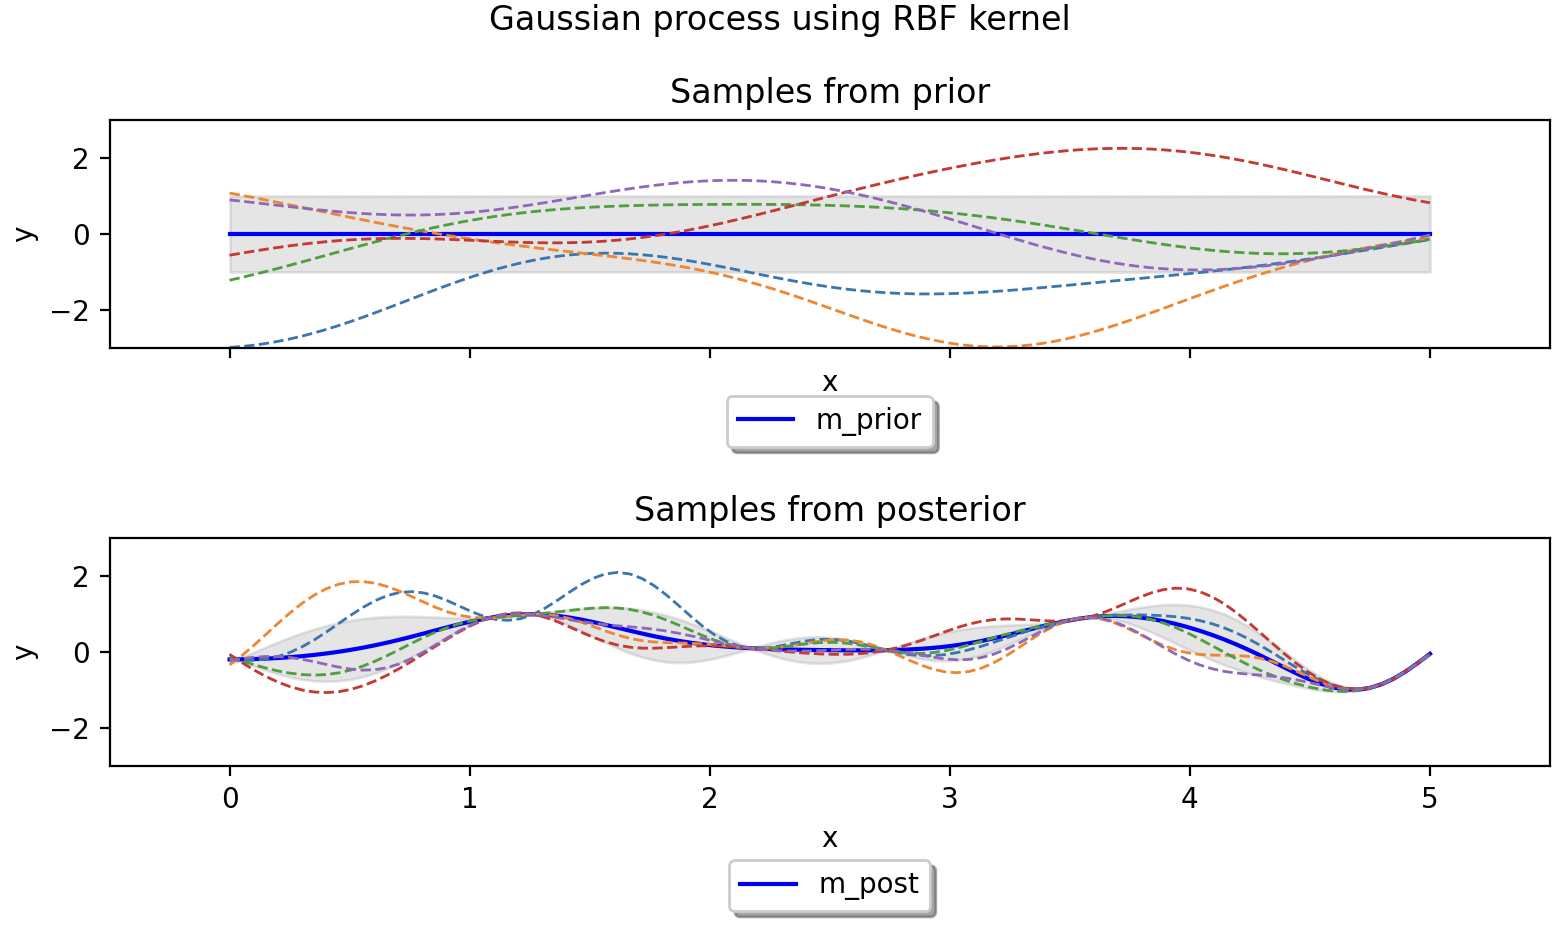
\includegraphics[width=1\textwidth]{img/prior_posterior}
    }

    The top plot represents the prior distribution.
    The mean line is flat and the uncertainty (shaded region) is uniform across the domain.
    This is because no observations are seen by the model yet, and all the parameters are initial.
    The samples are more diverse, showing wide range of possibilities.

    The bottom plot represents the posterior distribution.
    The model has been trained with the observations.
    The mean function now follows the trend of the data.
    The samples are more concentrated around the mean, showing less range of possibilities.
    The uncertainty band is narrower around observed regions and wider elsewhere, reflecting model confidence.

    \text{(l)}

    \centerline {
        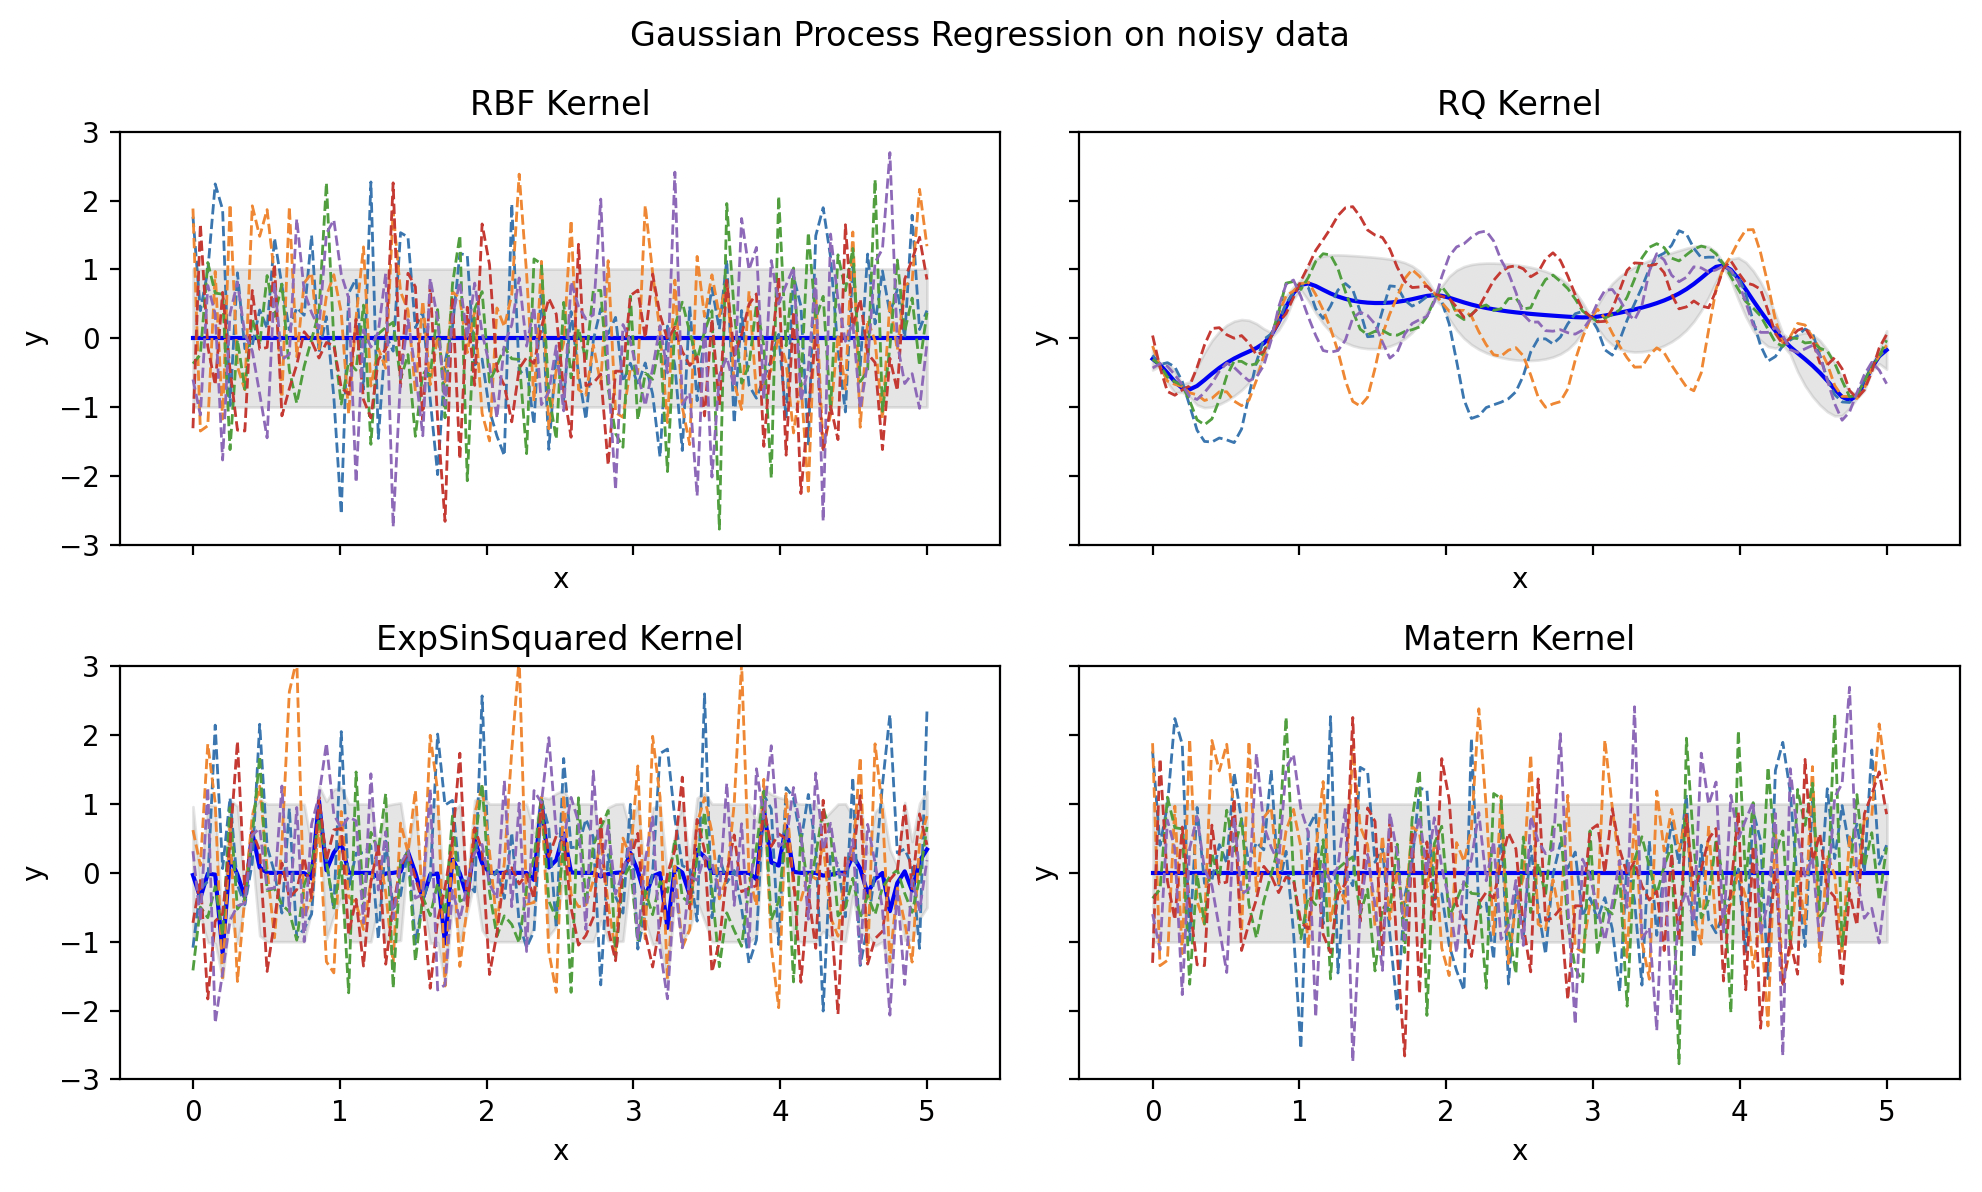
\includegraphics[width=1\textwidth]{img/four_kernels}
    }

    The \italic{Log Marginal Likelihood} for each kernel is:

    \begin{itemize}
        \item { RBF - $-11.0494$ }
        \item { Rational Quadratic - $-9.6207$ }
        \item { ExpSineSquared - $-9.1408$ }
        \item { Matern - $-11.0494$ }
    \end{itemize}

    The final length scale for each kernel is:

    \begin{itemize}
        \item { RBF - $0.38$ }
        \item { Rational Quadratic - $1^{-5}$ }
        \item { ExpSineSquared - $0.0878$ }
        \item { Matern - $1^{-5}$ }
    \end{itemize}

    The ExpSineSquared converges and yields the best Log Marginal Likelihood, so it is considered the best among the four kernels.

    The RQ (Rational Quadratic) kernel yields the second-best Log Marginal Likelihood, and its samples are narrower than other kernels'.
    However, its length scale is $1^{-5}$, meaning that it hasn't converged.
    This could be resulted from overfitting.

\end{solution}